% Chapter Template

\chapter{Filtering System in SLAMBench} % Main chapter title

\label{Chapter3} % Change X to a consecutive number; for referencing this chapter elsewhere, use \ref{ChapterX}

In this chapter, we propose two semantics of filtering system in SLAMBench to help us process input sensor frames. 
We describe the high-level architecture and how to perform a filtering task with two proposed filtering systems.

%----------------------------------------------------------------------------------------
%	SECTION 1
%----------------------------------------------------------------------------------------

\section{Overview}

Our filtering system takes two forms of a module which is separately defined for different filtering tasks (since we have found two types of filtering tasks that we could implement in SLAMBench). 
In C++, this can be achieved cleaning by declaring a header file (e.g., SLAMBenchFilterLibraryHelper.h) and using it to parameterize a filter module (e.g. identity filter).  
We conceive two filtering systems since so far, the filtering task for input sensor frames can be categorized into two forms: flow control and sensor modification. 

Originally, in the header file \code{SLAMBenchFilterLibraryHelper.h}, there are mainly three functions that help the user to configure a filter and run the filtering task

\begin{enumerate}
	\item \code{c\_sb\_new\_filter\_configuration} -  initialize the filter with the user-defined threshold parameter
	\item \code{c\_sb\_init\_filter} -  initialize sensors with \code{get\_sensors()} function to make sure that all sensors are found in the sensor library
	\item \code{c\_sb\_process\_filter} - ingest frame one by one with the sensors defined in the sensor library, process the frame in real time, and return the processed frame to the SLAMBench. 
	The frame is then ready to be sent to SLAM algorithms for mapping and localization. 
\end{enumerate}

If the user does not require the frame to be processed by batch (for example, the filtering system processes RGB frame, intensity frame and depth frame iteratively), or the user does not require the frame to be processed by updated sensors (for example, processing an resized frame requires a different sensor configuration from the original one), then this simple setting of filter (\ref{fig:filterarc}) works fine.

\begin{figure}[!htbp]
	\caption{\label{fig:filterarc}SLAMBench Original Filter Architecture}
	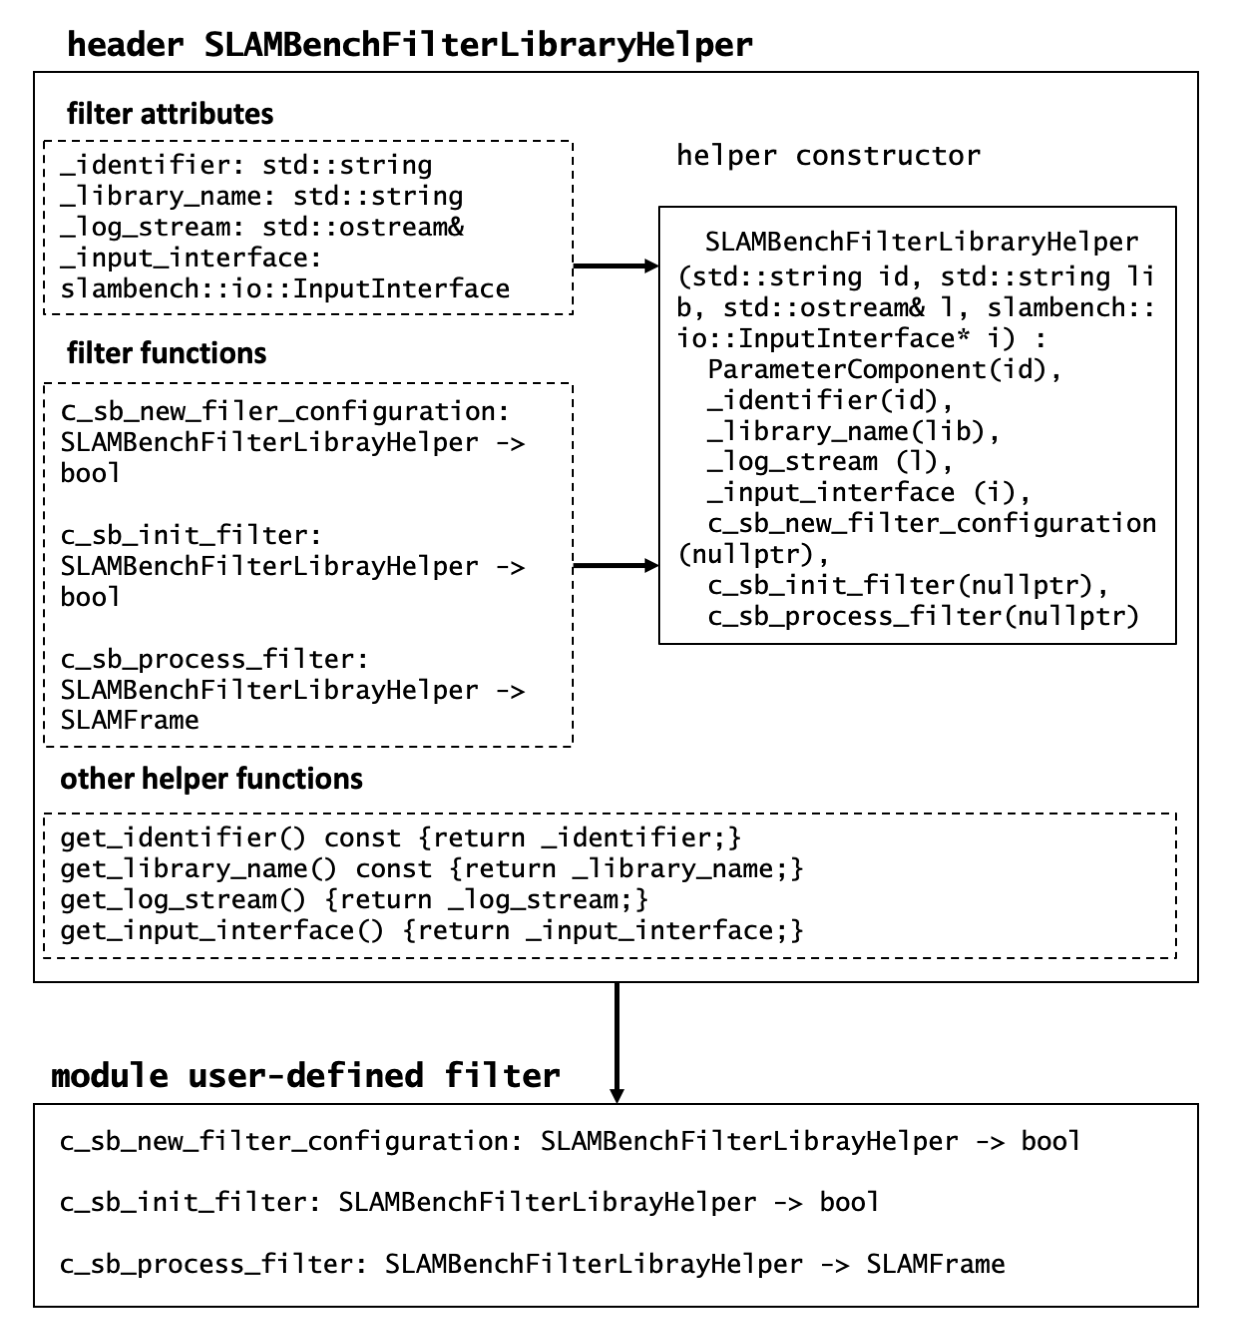
\includegraphics[width=14cm]{figures/filter-architecture.png}
	\centering
\end{figure}

However, for more complex (beyond single, size-fixed filtering task) filtering tasks, our filtering system cannot handle them. 
We need to restructure our filtering system, so that it can: 
\begin{enumerate}
	\item filter more than one frame at once, and
	\item modify the frame and ingest it with a software-defined sensor.
\end{enumerate}
Therefore, we have designed two filtering systems: flow filtering system and sensor filtering system.

%-----------------------------------
%	SECTION 2
%-----------------------------------

\section{Flow Filter}
Flow filter, as the name suggests, controls the flow of ingested frames. 
Before computing the frame, the SLAMBench loader calls functions in SLAMBench configurations to load libraries, datasets and sensors, retrieve ground truth and add performance metrics. 
After relevant objects of SLAMBench have been instantiated, the loader will start to compute frames in the \code{compute\_loop\_algorithm} function and iterate through frames one by one.

Then the current frame is passed to the filter. 
However, instead of processing the frame and directly returning the filtered frame to SLAMBench loader, the flow filter needs to hold the frame and decides whether the filter has enough frames to do multi-sensory filtering. 
If there are enough frames, then the flow filter starts to process all “buffered” frames (buffered in the sense that these frames have been stored in the flow filter with a time delayed state), and calls the SLAM algorithm to update filtered frames one by one. 
However, after a frame has been updated, the SLAM algorithm will also decide whether it has enough frames to process and generate a mapping output, so the SLAM algorithm will also hold on to the frames sent by filtered until sufficient frames have been passed in. 

Therefore, our flow filter needs to control the occurrence of four operations: 
\begin{enumerate}
	\item \code{input\_stream\_->GetNextFrame()} - when does the SLAMBench loader pass a new frame to filter;
	\item \code{c\_sb\_process\_filter} - when does the filter execute filtering task (this function will be created in the actual implementation;
	\item \code{c\_sb\_update\_frame\_filter} - when does the filter call the SLAM algorithm (lib) to update a frame;
	\item \code{c\_sb\_process\_once\_filter} - when does the filter call the SLAM algorithm (lib) to process the frames.
\end{enumerate}

And our flow filter needs to two conditional statements to control the flow of frames:
\begin{enumerate}
	\item \code{c\_sb\_buffer\_frame\_filter} - a function that ensures the filter has enough frames to do the processing, and returns a Boolean value;
	\item \code{c\_sb\_update\_frame\_filter} - – a function that returns Boolean value, notifying whether the SLAM algorithm has enough frames to start the processing.
\end{enumerate}

%-----------------------------------
%	SUBSECTION 2-1
%-----------------------------------
\subsection{Architectural Design \& Control Flow}

The flow filter is called when the SLAMBench loader calls the compute loop algorithm inside the SLAMBench Configuration. 
Therefore, the flow filter acts as a buffered interface between the SLAMBench Configurtation and a SLAM algorithm (\ref{fig:flowarc}).

\begin{figure}[!htbp]
	\caption{\label{fig:flowarc}Flow Filter Architecture}
	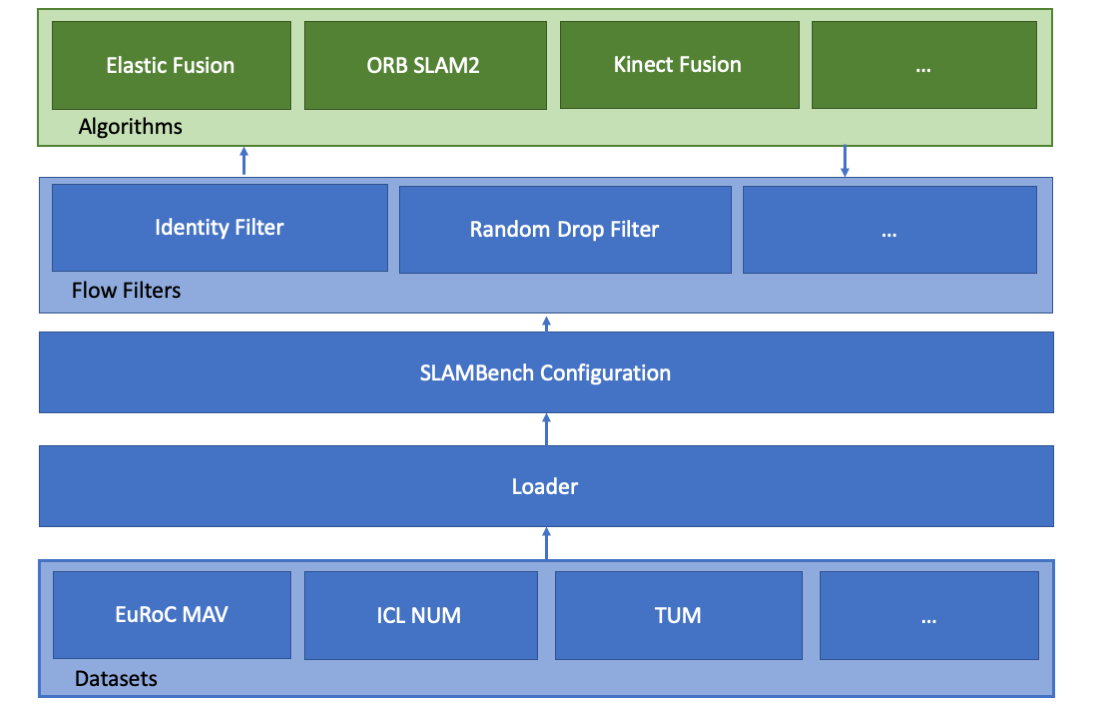
\includegraphics[width=14cm]{figures/flow-filter-architecture.png}
	\centering
\end{figure}

To control the flow of each sensor frame, and when it is filtered and processed, the flow filtering system executes the program in the following control flow diagram \ref{fig:controlflow}.

\begin{figure}[!htbp]
	\caption{\label{fig:controlflow}Flow Filter Control Flow Diagram}
	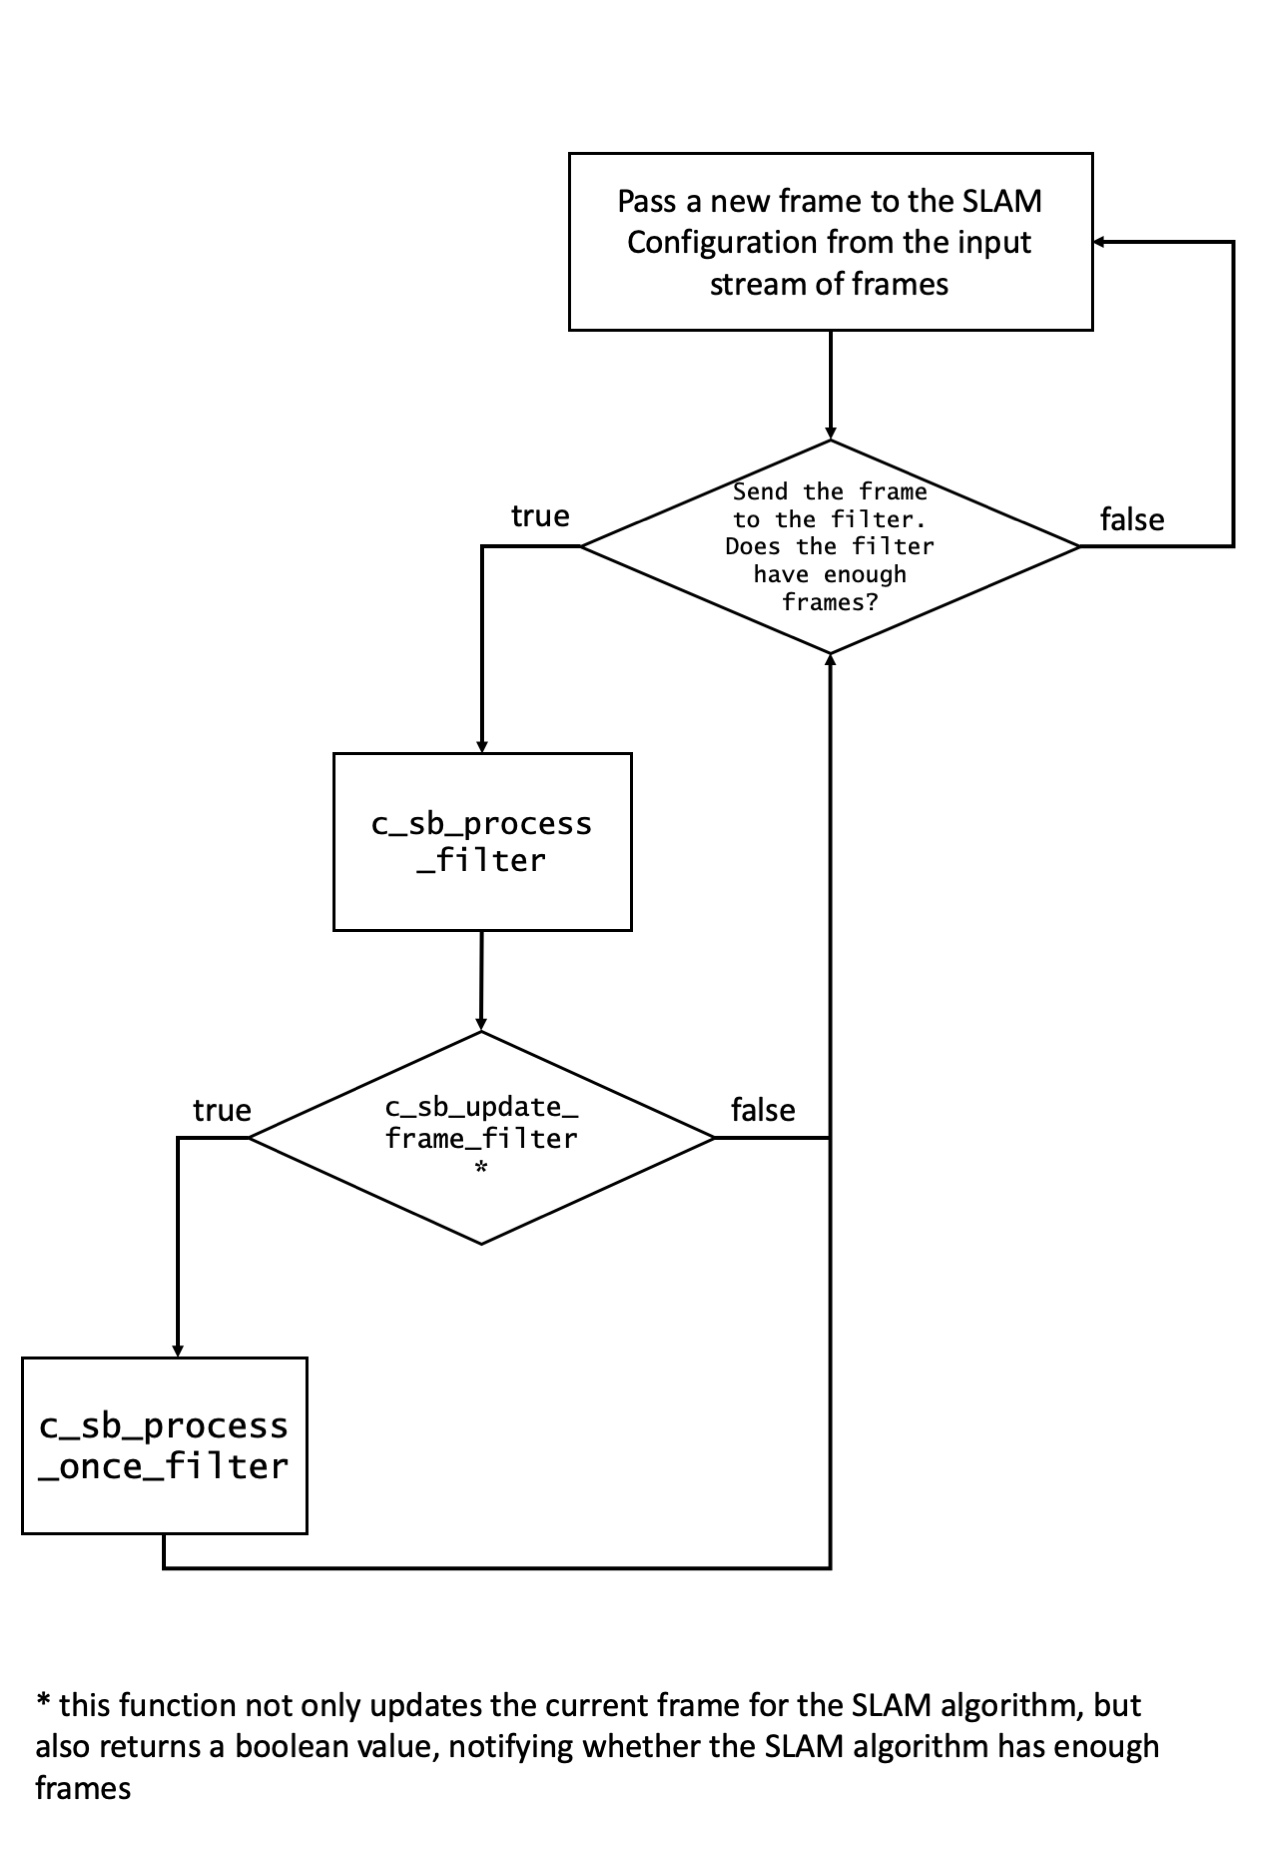
\includegraphics[width=12cm]{figures/control-flow-diagram.png}
	\centering
\end{figure}

\subsection{Multi-sensory Processing}

The main important reason to have a flow filter is to allow our filtering system to perform real-time multi-sensory processing. 
For our flow filter, it should be able to handle multiple frames from different sensors and process them at once in a delayed time state, since our flow filter can temporarily store frames, signals the SLAMBench Configuration and calls SLAM algorithm when stored frames have met a certain condition (e.g. sufficienet number of frames / types of frames, etc.). 

%-----------------------------------
%	SUBSECTION 2-2
%-----------------------------------
\subsection{Implementation}

In order to ensure that we can implement a flow filtering system inside the SLAMBench framework, we first construct an identity filter as a proof of concept. 
The identity filter is a middleware that ingests a sensor frame from the loader, make a copy of the frame and directly pass the copied frame to update the SLAM algorithm. 
Most of the work has been dedicating to revamping the \code{SLAMBenchFilteringLibraryHelper.h} and \code{SLAMBenchAPI.h} so that our identity filter can utilize functions from SLAMBench API, including \code{c\_sb\_update\_frame}, and \code{c\_sb\_process\_once} functions. 

The interaction of flow filtering for the identity filter is shown in the interaction diagram \ref{fig:flowinteract}. We note that there is complete transparency between the SLAMBench Configuration, Flow Filter, and the SLAM algorithm, in the sense that each component is informed the status of other components. 

\begin{figure}[!htbp]
	\caption{\label{fig:flowinteract}Identity Flow Filter Interaction Diagram}
	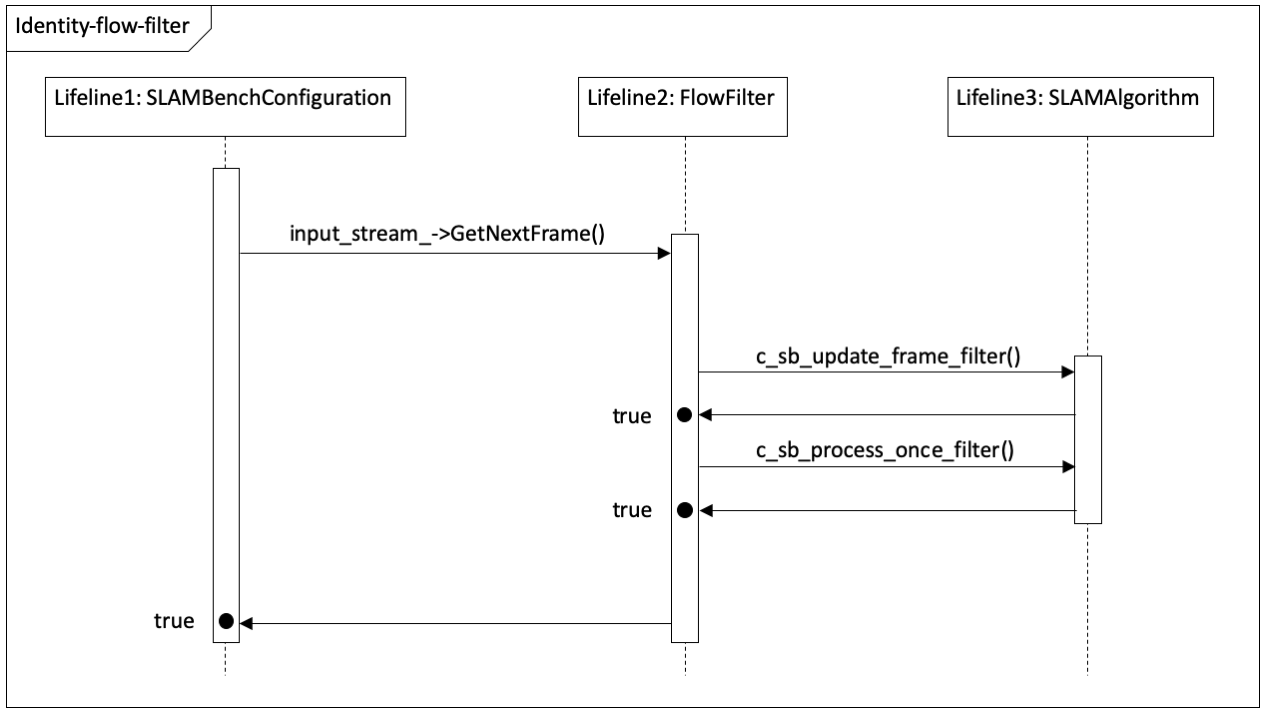
\includegraphics[width=14cm]{figures/interaction-diagram.png}
	\centering
\end{figure}

Now, to see that whether the identity filter actually produces the same frame, we have run the SLAMBench with different data sets and algorithms to test whether SLAMBench produce the same benchmarking results with and without the identity filter. Print message is also added in the identity filter to ensure that SLAMBench actually has passed frames to the identity filter. Indeed, after thorough testing, SLAM has passed the frame to the identity filter, and it produces the same result with and without the identity filter. 

%----------------------------------------------------------------------------------------
%	SECTION 3
%----------------------------------------------------------------------------------------

\section{Sensor Filter}

Sensor filter facilitates filtering tasks (e.g., resized, blurred, etc.) that requires another set of sensor, which allows the filtered frames to be processed by the SLAM algorithm. 
Therefore, for the sensor filter, we set the sensor configuration before initializing and configure the rest of the SLAMBench configuration. 

\begin{figure}[!htbp]
	\caption{\label{fig:sensorarc}Sensor Filter Architecture}
	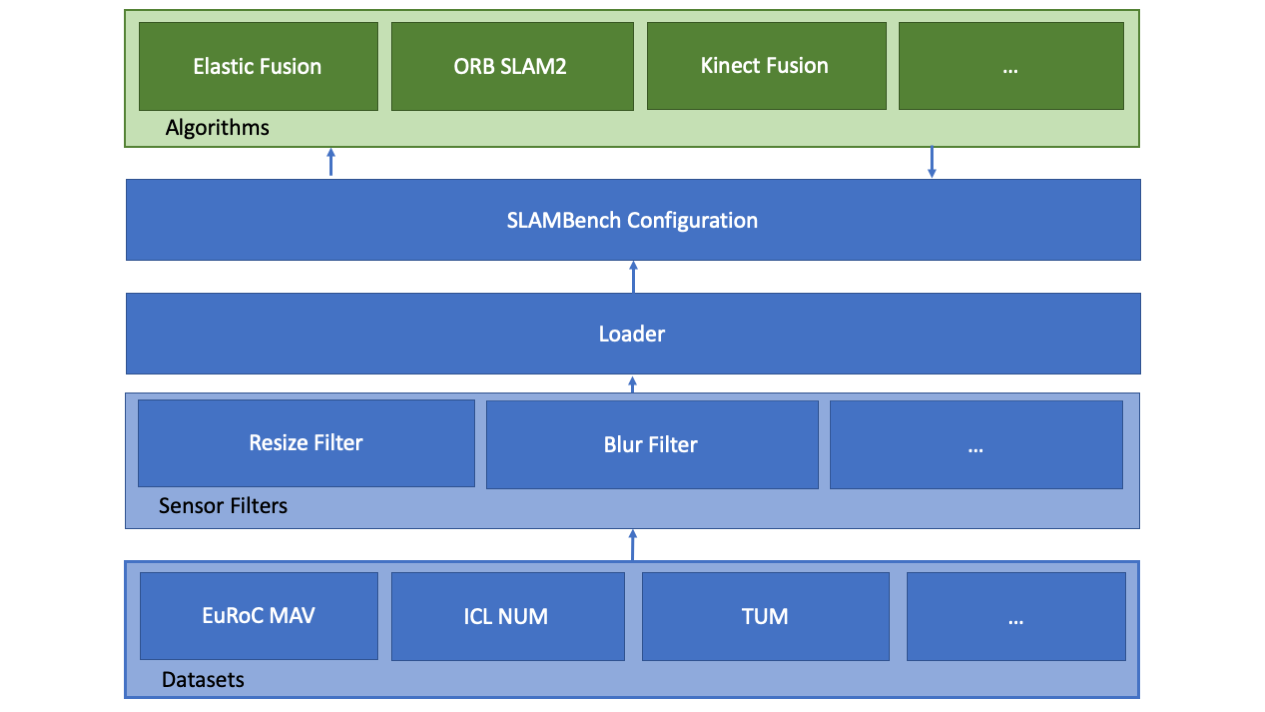
\includegraphics[width=14cm]{figures/sensor-filter-architecture.png}
	\centering
\end{figure}

However, this architecture would require the sensor filter to have a independent set of sensor object, which is challenging to implement within in the capstone period. Hence I will move on to implement the flow filter further and come back to the sensor filter if any other alternative architecture is possible.

%-----------------------------------
%	SUBSECTION 3-1
%-----------------------------------

%\subsection{Architectural Design}

%None yet.

%\subsection{Virtual Sensor}

%None yet.

